\documentclass[addpoints,12pt]{exam}

%\usepackage{newtxtext,newtxmath} % times new roman font
\usepackage{url}
\usepackage[dvipsnames]{xcolor}
\usepackage{enumitem}

\usepackage{bm,mathtools}
\DeclarePairedDelimiter\ceil{\lceil}{\rceil}

\usepackage{tikz}
\usetikzlibrary{shapes}

\usepackage{titling}
\setlength{\droptitle}{-6em}

\title{Midterm Exam \#1\\[0.25em]
\large CSC 485C/586C: Data Management on Modern Computer Architectures\\
Friday 14 February 2020, 10.35-11.20}
\date{}

\begin{document}
\maketitle

\vspace{-6.5em}
{\centering
  \hspace{0.05\textwidth}
  \parbox{0.6\textwidth}{%
    Name:\enspace\hrulefill
  }\hspace{2em}
  \parbox{0.25\textwidth}{%
    V00\enspace\hrulefill
  }
}

\bigskip
%\printanswers
\begin{questions}
 \question Please explain the following concepts in 1-3 sentences and/or code snippets and/or a small illustration.  An excellent answer does not have to be long, just precise.\\{\em Guide: 2 minutes each} 

 \medskip
 
 \begin{parts}
   \part[1] Bad Speculation
     \begin{solution}[6em]
     \end{solution}
   
   \part[1] Cold Data
     \begin{solution}[6em]
     \end{solution}
   
   \part[1] Latency
     \begin{solution}[6em]
     \end{solution}
   
   \part[1] Locality of Reference
     \begin{solution}[6em]
     \end{solution}
   
   \part[1] Memory-Bond
     \begin{solution}[6em]
     \end{solution}
 \end{parts}
 
 \newpage
 \question You have a contiguously laid out, sequential linked list in which each node of the linked list is defined as follows:

\begin{verbatim}
struct Node
{
    Node *next;
    char padding[ npad ]; // npad is a constant defined elsewhere
};
\end{verbatim}

Answer the following questions that analyse this figure below (taken from Drepper):\\
{\em Guide: 10 min total}

\hspace{0.2\textwidth}\parbox{0.6\textwidth}{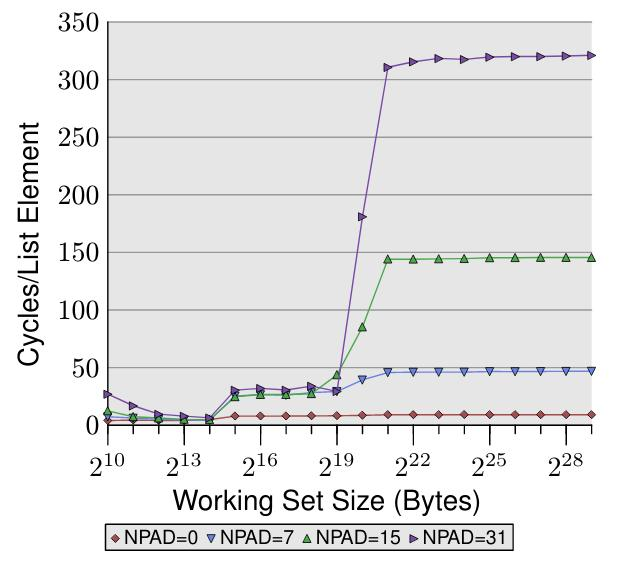
\includegraphics[ scale = 0.5]{fig/drepper-wss.jpg}}


   \begin{parts}
       \part[2] What does the shape of the trendlines indicate?
           \begin{solution}[5em]
           \end{solution}

       \part[2] Why does the curve corresponding to \texttt{npad=0} appear not to have the same shape as the other curves?
           \begin{solution}[5em]
           \end{solution}

       \part[2] What is the overall message (a.k.a., purpose, or significance) of the plot?
           \begin{solution}[5em]
           \end{solution}
   \end{parts}
 
 
  \question[8] A "Palentine's Card" is a warm greeting card that one gives to a friend on 14 February. Below we have a data structure to define a set of Paletine's Cards and an algorithm to count how many pairs have the same sender {\em and} recipient, i.e., cases where one person gave multiple cards to the same pal. Sadly, the code suffers from poor cache performance. Rewrite both the data structures and implementation to optimise cache performance. (Pseudocode or annotations is fine; proper syntax is not evaluated, so long as the intent is clear.)\\
{\em Guide: 15 min}
  
   \bigskip
    \begin{minipage}{.4\textwidth}
      \begin{verbatim}
struct palentine
{
  std::string sender_name;
  std::string recipient_name;
  std::string message;
};

// overload == for palentine
bool operator == ( /*...*/ )
{
    // return true if both sender
    // and recipient match
}

std::vector< palentine > cards;
      \end{verbatim}
    \end{minipage}
    \hfill
    \begin{minipage}{.5\textwidth}
      \begin{verbatim}
template < typename T >
auto num_matching_cards( T const& cards )
{
    auto const n = cards.size();
    auto num_matches = 0llu;

    for( auto i = 0u; i < n; ++i )
    {
        for( auto j = i + 1; j < n; ++j )
        {
            if( cards[ i ] == cards[ j ] )
                ++num_matches;
        }
    }
    return num_matches;
};
      \end{verbatim}
    \end{minipage}
    

      \begin{solution}[15em]
      \end{solution}
    
    \newpage
    \question[2] How would you verify that your optimisations to \texttt{num\_matching\_cards()} improved cache performance?\\
{\em Guide: 5 min}
      
      \begin{solution}[5em]
      \end{solution}


    \question Answer the following two questions on the data structure below:\\
{\em Guide: 5 min}

\begin{verbatim}
struct box_of_chocolates
{
    uint16_t num_milk_chocolates;
    uint16_t num_dark_chocolates;
    uint8_t  num_white_chocolates;
    uint32_t box_size; // volume in cubic millimeters
};
\end{verbatim}

      \begin{parts}
         \part[2] Considering alignment, how would you change this struct without changing any data types so that your working set size was reduced?\\
      
      \begin{solution}[8em]
      \end{solution}

         \part[1] How would you verify that your changes had reduced the working set size?\\
      
      \begin{solution}[5em]
      \end{solution}
    
      \end{parts}
\end{questions}

\vfill
\begin{minipage}{.2\textwidth}\hphantom{xxxxxxxxxxx}\end{minipage}
\gradetable[h][questions]

\end{document}
